\titleformat {\chapter} {\normalfont\huge\bfseries\color{black}}   {\thechapter}{10pt}{\huge} 
\chapter {Functional and Behavioral Designs}

\section{Interaction View Point}
\subsection{Activity Diagram 1}


\vspace*{1\baselineskip}
\begin{figure}[htbp]
	\begin{center}
		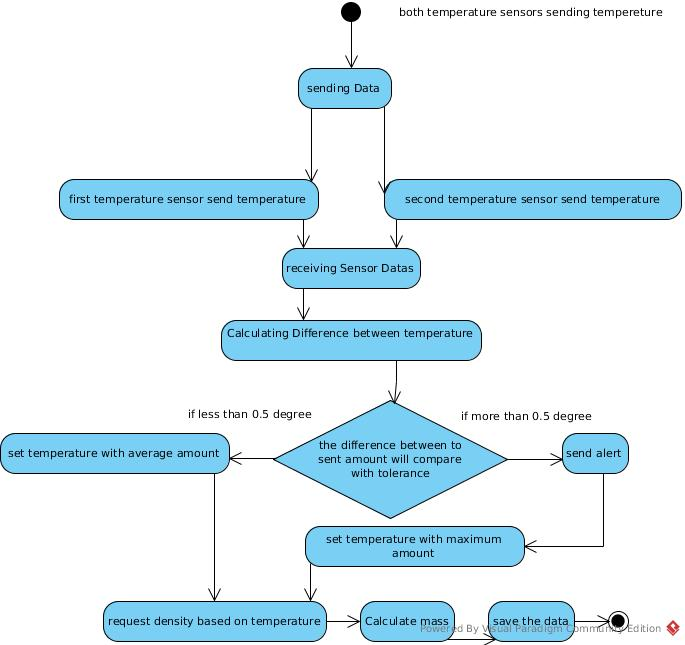
\includegraphics[width=1.00\linewidth]{./images/AD.jpg}
		\caption{Activity diagram for conversion calculation.}
		\label{fig:AD.jpg}
	\end{center}
\end{figure}

\subsubsection{Description}

\vspace*{1\baselineskip}
\noindent{
	Based on figure B.1,Two temperature sensors send the last temperatures to system and system checks differences between the amount of both.if the difference more than 0.5 degree then system send alert because of security in tank,it will set the maximum amount between them as temperature amount,else it will set the average based on the new temperature and product id.It will find the density and calculate the mass\\}


\newpage
\subsection{Activity Diagram 2}
\vspace*{1\baselineskip}
\begin{figure}[htbp]
	\begin{center}
		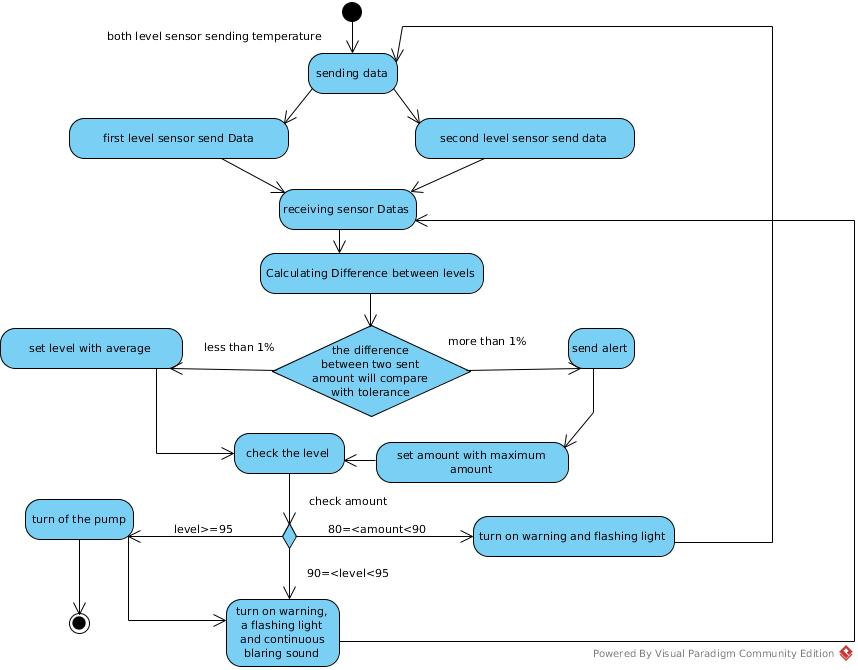
\includegraphics[width=1.00\linewidth]{./images/AD1.jpg}
		\caption{Activity diagram for Handling Rising Tank Levels.}
		\label{fig:AD1.jpg}
	\end{center}
\end{figure}

\subsubsection{Description}

\vspace*{1\baselineskip}
\noindent{
	Based on figure B.2,The system receive data from both level sensor. the system will calculate difference between levels. Once difference is calculated then average amount is set.  The system checks the level. If the amount is more than 80 and less than 90, system will turn on warning and flashing light. If the amount is more than 90 and less than 95, system will turn on warning, flashing light and continuous sound. If the amount more than 95, the system will turn off pump.\\}



\newpage
\subsection{Sequence Diagram 1}
\vspace*{1\baselineskip}
\begin{figure}[htbp]
	\begin{center}
		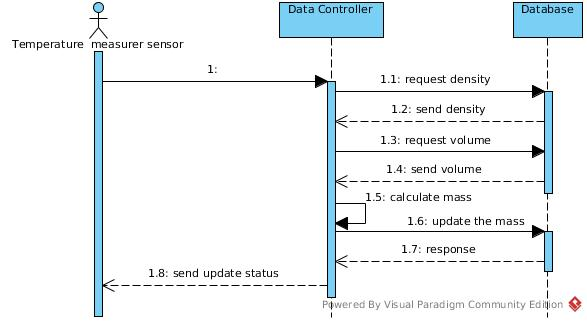
\includegraphics[width=1.00\linewidth]{./images/SeDiagram.jpg}
		\caption{Sequence diagram for conversion calculation.}
		\label{fig:SeDiagram.jpg}
	\end{center}
\end{figure}

\subsubsection{Description}
\vspace*{1\baselineskip}
\noindent{
	Based on figure B.3,The sensors will send the level .the Data Controller will check this amount and it will request the density from database, based on this density it will calculate the mass and save it to the database.\\}

\newpage
\subsection{Sequence Diagram 2}
\vspace*{1\baselineskip}
\begin{figure}[htbp]
	\begin{center}
		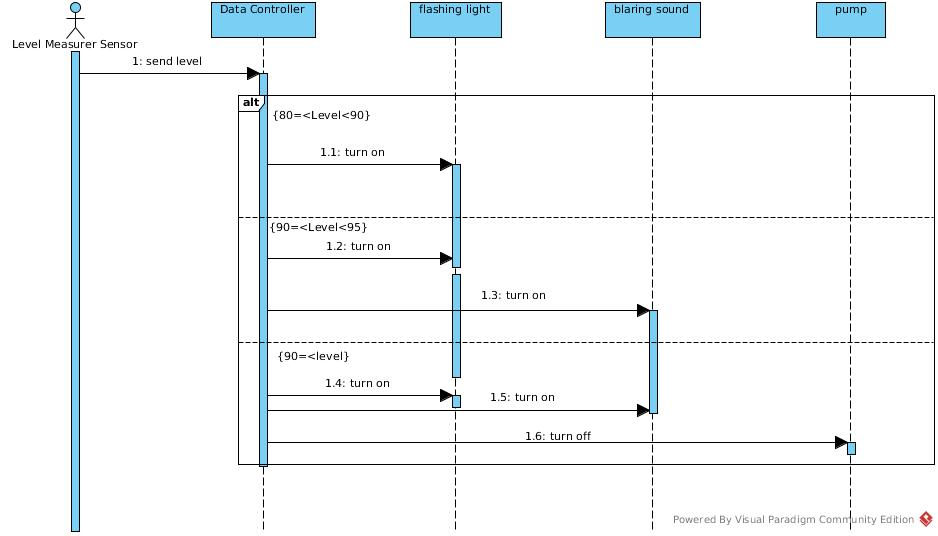
\includegraphics[width=1.00\linewidth]{./images/SeDiagram1.jpg}
		\caption{Sequence diagram for Handling Rising Tank Levels.}
		\label{fig:SeDiagram1.jpg}
	\end{center}
\end{figure}

\subsubsection{Description}
\vspace*{1\baselineskip}
\noindent{
	Based on figure B.4,The sensors will send the level .the Data Controller will check this amount and will turn on the flashing light if (80=$<$level$<$90),will turn on both flashing light and alarm if (90=$<$level$<$95) and at the end it also will turn off the pump.\\}



\newpage
\subsection{Activity Diagram For Notification}
\vspace*{1\baselineskip}
\begin{figure}[htbp]
	\begin{center}
		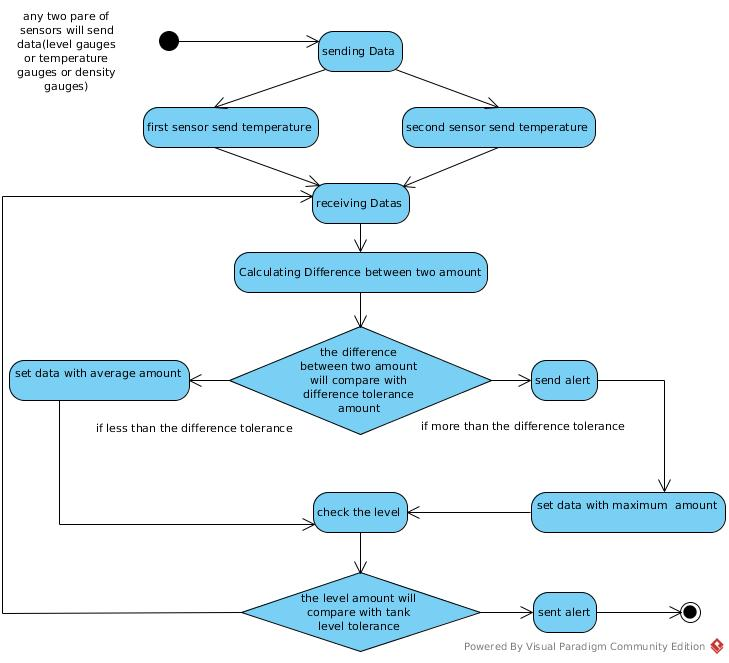
\includegraphics[width=1.00\linewidth]{./images/Notify.jpg}
		\caption{Activity diagram for notification in Tank Farm Inventory System.}
		\label{fig:Notify.jpg}
	\end{center}
\end{figure}

\subsubsection{Description}

\vspace*{1\baselineskip}
\noindent{
	Based on figure B.5, after any Two pair of  sensors send the last  data to the system. The system will  check the difference between the amount of both, if the difference be more than tolerance  the system will send sms, email, hats app and telegram message  then because of security issue  in the tank it will set the maximum amount between them as  amount, else it will set the average .based in the new level amount it will compare this amount with three different situation and will send  sms,email,whats app and telegram message in case of violating tolerance \\}


\newpage
\subsection{State Dynamics View Point}
\subsubsection{State transition diagram 1}

\vspace*{1\baselineskip}
\begin{figure}[htbp]
	\begin{center}
		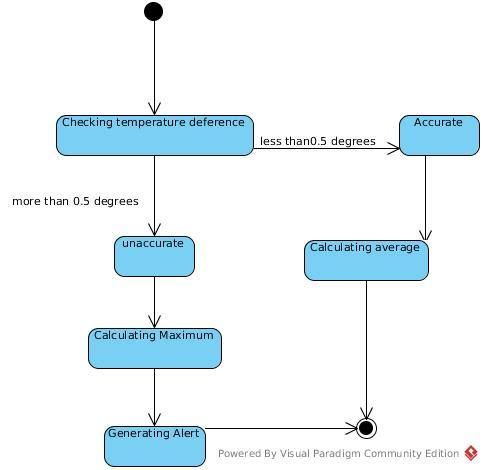
\includegraphics[width=0.40\linewidth]{./images/State1.jpg}
		\caption{State transition diagram for temperature state.}
		\label{fig:State1.jpg}
	\end{center}
\end{figure}

\subsubsection{Description}

\vspace*{1\baselineskip}
\noindent{
	Based on figure B.6,the system will check the difference and will go to accurate state in case of no violating the tolerance else  will go to inaccurate state after each one will calculating maximum and generating alert.\\}

\newpage
\subsubsection{State transition diagram 2}
\vspace*{1\baselineskip}
\begin{figure}[htbp]
	\begin{center}
		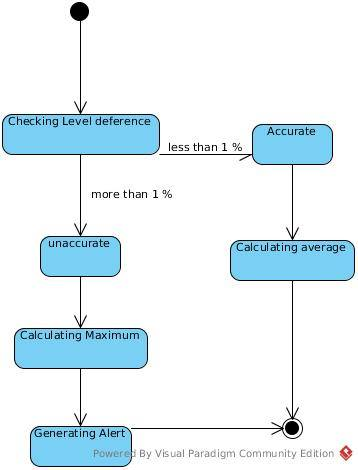
\includegraphics[width=0.40\linewidth]{./images/State2.jpg}
		\caption{State transition diagram for level state.}
		\label{fig:State2.jpg}
	\end{center}
\end{figure}

\subsubsection{Description}

\vspace*{1\baselineskip}
\noindent{
	Based on figure B.7,the system will check the level difference and will go to accurate state in case of no violating the tolerance else  will go to inaccurate state after each one will calculating maximum and generating alert.\\}

\newpage
\subsubsection{State transition diagram 3}
\vspace*{1\baselineskip}
\begin{figure}[htbp]
	\begin{center}
		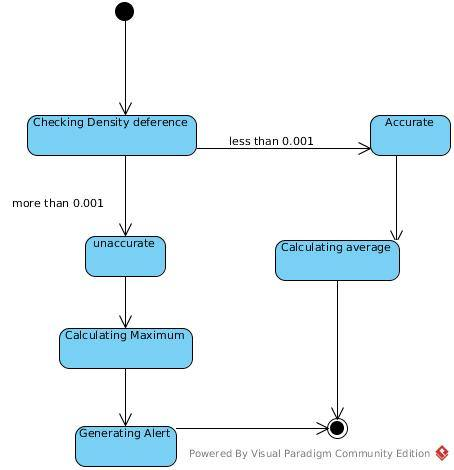
\includegraphics[width=0.40\linewidth]{./images/State3.jpg}
		\caption{State transition diagram for density state.}
		\label{fig:State3.jpg}
	\end{center}
\end{figure}

\subsubsection{Description}

\vspace*{1\baselineskip}
\noindent{
	Based on figure B.8,the system will check the density difference and go to accurate state in case of no violating the tolerance else the system will go to inaccurate state after each one will calculating maximum and generating alert.\\}

